
\documentclass[12pt,a4paper]{report}
\usepackage[utf8]{inputenc}
\usepackage[T1]{fontenc}
\usepackage[margin=1in]{geometry}
\usepackage{graphicx}
\usepackage{amsmath,amssymb}
\usepackage{tabularx}
\usepackage{booktabs}
\usepackage{float}
\usepackage{setspace}
\usepackage{verbatim}
\usepackage{enumitem}
\usepackage{xcolor}
\usepackage{array}
\usepackage{multirow}
\usepackage{adjustbox}
\usepackage{listings}
\usepackage{caption}
\usepackage{subcaption}
\usepackage{tcolorbox}
\usepackage{fancyhdr}
\usepackage{titlesec}
\usepackage{mdframed}
\usepackage[colorlinks=true, linkcolor=blue, citecolor=blue, urlcolor=blue]{hyperref}
\usepackage{pmboxdraw}
\usepackage{tikz}
\usetikzlibrary{positioning, shapes.geometric, arrows.meta, backgrounds, fit, arrows}

% ---- Counter setup ----
\counterwithout{equation}{chapter}
\counterwithout{figure}{chapter}
\counterwithout{table}{chapter}

\onehalfspacing

% ---- Listing style ----
\lstset{
  basicstyle=\ttfamily\small,
  backgroundcolor=\color{gray!10},
  frame=single,
  breaklines=true,
  keywordstyle=\color{blue}\bfseries,
  commentstyle=\color{green!60!black},
  stringstyle=\color{red!70!black},
  numbers=left,
  numberstyle=\tiny\color{gray},
  xleftmargin=2em
}

% ---- tcolorbox styles ----
\tcbuselibrary{skins, breakable}
\newtcolorbox{infobox}[1][]{
  colback=blue!5!white, colframe=blue!60!black,
  fonttitle=\bfseries, title=#1,
  breakable
}
\newtcolorbox{formulabox}{
  colback=yellow!10!white, colframe=orange!80!black,
  fonttitle=\bfseries, breakable
}

% ---- Header/footer ----
\pagestyle{fancy}
\fancyhf{}
\fancyhead[L]{\small AI-Powered Business Intelligence System}
\fancyhead[R]{\small Amrita Vishwa Vidyapeetham}
\fancyfoot[C]{\thepage}
\renewcommand{\headrulewidth}{0.4pt}

\begin{document}

% ==============================================================
%  COVER PAGE
% ==============================================================
\begin{titlepage}
\begin{center}
\vspace*{0.5cm}
{\Large \bfseries AI-Powered Business Intelligence System:\\[0.3cm]
Large Aspect-Based Sentiment Analysis and\\[0.2cm]
Decision Support Platform\par}

\vspace{1.2cm}
A Dissertation submitted in partial fulfillment\\
of the requirements for the degree\\
of\\

\vspace{0.4cm}
{\Large \bfseries INTEGRATED MASTER OF SCIENCE \par}
{\large \bfseries IN\par}
{\large \bfseries DATA SCIENCE\par}

\vspace{0.4cm}
by\\[0.3cm]
{\large \bfseries SUNDARA THAMIZHAN\par}
{\large \bfseries CB.PS.I5DAS22055\par}

\vspace{1.2cm}
\includegraphics[width=0.75\textwidth]{cover logo.png}

\vspace{1.2cm}
{\large \bfseries DEPARTMENT OF MATHEMATICS\par}
{\large \bfseries AMRITA SCHOOL OF PHYSICAL SCIENCES\par}
{\large \bfseries AMRITA VISHWA VIDYAPEETHAM\par}
\vspace{0.2cm}
{\small COIMBATORE -- 641\,112 (INDIA)\par}
\vspace{0.2cm}
{\bfseries April 2026\par}
\end{center}
\end{titlepage}

% ==============================================================
%  BONAFIDE CERTIFICATE
% ==============================================================
\newpage
\thispagestyle{empty}
\begin{center}
{\large \bfseries AMRITA SCHOOL OF PHYSICAL SCIENCES\par}
\vspace{0.3cm}
{\Large \bfseries AMRITA VISHWA VIDYAPEETHAM\par}
\vspace{0.2cm}
{\small COIMBATORE -- 641\,112\par}

\vspace{0.6cm}
\includegraphics[width=0.75\textwidth]{cover logo.png}

\vspace{0.6cm}
{\Large \bfseries BONAFIDE CERTIFICATE\par}
\end{center}
\vspace{0.4cm}

\noindent This is to certify that the dissertation entitled
\textbf{``AI-Powered Business Intelligence System: Large Aspect-Based Sentiment
Analysis and Decision Support Platform''} submitted by
\textbf{SUNDARA THAMIZHAN (Reg.\ No.: CB.PS.I5DAS22O55)}, for the award of
the \textbf{Degree of Integrated Master of Science} in \textbf{Data Science}
is a bonafide record of the work carried out by him at the Department of
Mathematics, Amrita School of Physical Sciences, Amrita Vishwa Vidyapeetham,
Coimbatore.

\vspace{3cm}
\noindent
\begin{tabular}{@{}p{0.5\linewidth} p{0.5\linewidth}@{}}
Signature of Examiner & Signature of Project Coordinator \\[2.5cm]
& \\
\end{tabular}

\vspace{1.5cm}
\begin{center}
Signature of Chairperson
\end{center}

% ==============================================================
%  DECLARATION
% ==============================================================
\newpage
\begin{center}
{\large \bfseries AMRITA SCHOOL OF PHYSICAL SCIENCES\par}
\vspace{0.3cm}
{\Large \bfseries AMRITA VISHWA VIDYAPEETHAM\par}
\vspace{0.2cm}
{\small COIMBATORE - 641 112\par}
\vspace{0.3cm}
{\large \bfseries DEPARTMENT OF MATHEMATICS\par}
\vspace{0.8cm}
{\Large \bfseries DECLARATION\par}
\end{center}
\vspace{0.5cm}

\noindent I, \textbf{SUNDARA THAMIZHAN (Reg.\ No.: CB.PS.I5DAS22O55)},
hereby declare that this dissertation entitled
\textbf{``AI-Powered Business Intelligence System: Large Aspect-Based Sentiment
Analysis and Decision Support Platform''} is the record of the original work
done by me at the Department of Mathematics, Amrita School of Physical Sciences,
Amrita Vishwa Vidyapeetham, Coimbatore. To the best of my knowledge, this work
has not formed the basis for the award of any degree, diploma, associateship,
fellowship, or similar title to any candidate in any University.

\vspace{2cm}
\noindent
\begin{tabular}{@{}p{0.5\linewidth} p{0.5\linewidth}@{}}
Place: Coimbatore & \hfill Signature of the Student \\[0.8cm]
Date: \phantom{Coimbatorexx} & \\
\end{tabular}

\vspace{3cm}
\begin{center}
\textbf{COUNTERSIGNED}\\[0.8cm]
\textbf{Dr.\ Sangeeta Kumari}\\
Project Coordinator\\
Department of Mathematics\\
Amrita School of Physical Sciences
\end{center}

% ==============================================================
%  ACKNOWLEDGEMENT
% ==============================================================
\newpage
\chapter*{Acknowledgement}
\addcontentsline{toc}{chapter}{Acknowledgement}

I sincerely extend my gratitude to my project coordinator, \textbf{Dr.\ Sangeeta Kumari}, Department of Mathematics, Amrita School of Physical Sciences, Amrita Vishwa Vidyapeetham, for her constructive guidance, consistent encouragement, and invaluable mentorship throughout the execution of this research project. Her critical observations at every stage helped sharpen both the technical depth and the academic presentation of this work.

I deeply thank the \textbf{Head of the Department of Mathematics} alongside all faculty members for cultivating a supportive and research-oriented academic environment within the department. Their pedagogical commitment gave me the disciplinary tools required to tackle complex problems in data science and natural language processing. My appreciation equally extends to my peers and friends who contributed through technical brainstorming sessions, user-testing the application interface, and offering timely suggestions when specific design decisions required external perspectives.

I acknowledge the transformative contributions of the open-source community, particularly the maintainers behind \textbf{HuggingFace Transformers}, \textbf{Streamlit}, \textbf{PyTorch}, \textbf{scikit-learn}, and \textbf{Groq}. Their robust, well-documented frameworks provided the foundational infrastructure upon which this entire project is constructed. The shared culture of openness in the machine learning community continues to democratize access to advanced artificial intelligence capabilities.

Finally, my deepest appreciation is reserved for my family, whose unwavering moral support and patient understanding sustained my academic commitment through every demanding phase of this programme.

\vspace{2cm}
\begin{flushright}
\textbf{SUNDARA THAMIZHAN}\\
\textbf{CB.PS.I5DAS22O55}
\end{flushright}

% ==============================================================
%  ABSTRACT
% ==============================================================
\newpage
\chapter*{Abstract}
\addcontentsline{toc}{chapter}{Abstract}

Unstructured customer feedback distributed across diverse digital platforms offers vital intelligence regarding consumer behavior and product viability. However, systematically processing this information at scale involves technical challenges that remain largely inaccessible to small and medium enterprises (SMEs). This dissertation proposes an AI-Powered Business Intelligence System—a fully integrated Software-as-a-Service (SaaS) platform designed to distill raw customer reviews into interpretable strategic directives suitable for non-technical business decision-makers.

Central to the architecture is an Aspect-Based Sentiment Analysis (ABSA) module, constructed using a fine-tuned BERT model operating on text-pair inputs. The analyzer isolates and scores customer feedback against four operationally relevant dimensions: Product, Service, Price, and Ambience. To maintain robust prediction transparency, the system incorporates an Explainable AI (XAI) workflow featuring token-level attention visualizations alongside a computationally efficient Leave-One-Out (LOO) attribution method that approximates SHAP score computations without the associated memory overhead.

Working in tandem, an ensemble Random Forest classifier continuously generates customer churn risk estimates from extracted sentiment indicators. A cloud-hosted large language model (Groq LLaMA 3.1-8B-Instant) complements these predictions by composing customized response messages and generating concise executive analytical reports. The system additionally incorporates live social media tracking by aggregating Twitter/X and Google Play review data, Latent Dirichlet Allocation (LDA) for thematic complaint discovery, and visual benchmarking of direct market competitors through interactive radar charts. Evaluative testing confirms high classification performance across all four aspects, and batch processing experiments demonstrate a hardware throughput improvement of approximately 33 times over equivalent sequential execution patterns.

\vspace{0.5cm}
\noindent\textbf{Keywords:} Aspect-Based Sentiment Analysis, BERT, Business Intelligence, Explainable AI, SHAP, Random Forest, Churn Prediction, Streamlit, NLP, SaaS, Zero-Shot Classification, LDA, Groq LLM, Leave-One-Out Attribution.

% ==============================================================
%  TABLE OF CONTENTS
% ==============================================================
\newpage
\tableofcontents

\newpage
\listoffigures
\listoftables

% ==============================================================
%  CHAPTER 1 — INTRODUCTION
% ==============================================================
\chapter{Introduction}
\thispagestyle{fancy}

\section{Background and Motivation}
Consumer feedback distributed across digital ecosystems—ranging from localized review aggregators to large-scale social media conversations—provides key indicators of business operational health. Established enterprises equipped with dedicated data science divisions systematically capture and leverage these signals for competitive advantage. Conversely, small and medium enterprises routinely lack the technical personnel, infrastructure budget, or domain knowledge required to decode this volume of textual information effectively. Manually reading thousands of monthly reviews is practically unscalable, inherently susceptible to confirmation bias, and introduces significant interpretive fatigue among operational managers.

General-purpose sentiment analysis tools fail to adequately address this bottleneck. Most commercially available products classify documents simply as positive, negative, or neutral. This broad categorization obscures the granular meaning embedded within customer narratives. A patron might compose a highly positive review regarding food taste while simultaneously criticizing waiting times and pricing strategy. Discerning the precise origin of customer dissatisfaction demands Aspect-Based Sentiment Analysis (ABSA)—a methodological evolution that separates and individually classifies opinions focused on distinct, operationally meaningful business dimensions.

The business intelligence gap is most acute within the restaurant, hospitality, and retail sectors, where product quality, service delivery, pricing perception, and environmental ambience collectively shape customer retention. Survey-based feedback collection presents additional challenges: response rates remain low, survey fatigue distorts results, and the inherently structured format of questionnaires prevents customers from expressing compound opinions that naturally arise during real service encounters. Mining existing organic review data from public digital platforms offers a more authentic and continuously refreshed alternative.

\section{Problem Definition}
This project addresses the challenge of designing, engineering, and deploying an automated business intelligence application that overcomes persistent technical barriers facing SME operators. Specifically, the proposed system aims to ingest scattered textual reviews from multiple sources and deliver focused, explainable, and actionable sentiment predictions. It systematically resolves five distinct operational challenges:

\begin{enumerate}[leftmargin=2em]
  \item \textbf{Aspect Detection:} Reliably determining whether any given piece of text addresses product quality, service delivery, pricing fairness, or environmental atmosphere—without depending on manually annotated domain-specific training datasets.
  \item \textbf{Aspect Classification:} Attaching accurate sentiment polarity labels to each detected business dimension with transparent confidence scoring.
  \item \textbf{Algorithmic Explainability:} Ensuring that individual predictions can be clearly understood by non-technical managers through token-level visualization that reveals exactly which words drove each classification outcome.
  \item \textbf{Attrition Estimation:} Translating qualitative narrative feedback into a statistically grounded customer churn risk coefficient that feeds into CRM workflows.
  \item \textbf{Strategic Application:} Converting computationally identified problems into directly executable business improvement recommendations delivered through automated LLM-generated advisory reports.
\end{enumerate}

\section{Proposed System Overview}
The resulting architecture, named \textbf{BizDecisions AI}, is a modular multi-tab web application managed through the Streamlit framework. It organizes analytical functionality into six distinct user-facing layers:

\begin{itemize}[leftmargin=2em]
  \item \textbf{Tab 1 -- Single Review Analyzer:} An isolated processing environment for granular per-review analysis with full XAI visualization output.
  \item \textbf{Tab 2 -- Bulk CSV Processor:} High-throughput batch processing supporting up to 500 review entries concurrently, triggering automated LDA topic clustering on completion.
  \item \textbf{Tab 3 -- Model Evaluator:} Provides statistical validation metrics against pre-labeled test datasets uploaded by the operator, presenting classification reports and confusion matrices.
  \item \textbf{Tab 4 -- Weekly AI Report:} Fuses LLM-generated executive advisory summaries with numeric business health indicators into exportable PDF reports.
  \item \textbf{Tab 5 -- Social Media Monitor:} Continuously aggregates inbound textual data from Twitter/X and Google Play Store reviews for real-time operational awareness.
  \item \textbf{Tab 6 -- Competitor Comparison:} Benchmarks internal sentiment metrics against identified competitor entities using dynamic radar chart visualization.
\end{itemize}

\section{Objectives}
The primary goals directing this research include: (i) engineering a robust ABSA pipeline exploiting text-pair encoding to maximize cross-attention between opinion spans and target aspect labels; (ii) integrating a comprehensive explainable AI toolkit that democratizes model transparency for non-specialist users; (iii) implementing proactive churn risk quantification through a Random Forest ensemble trained on derived sentiment features; and (iv) unifying these analytical components with LLM-powered report generation within a secured, session-aware SaaS framework suitable for live multi-tenant deployment.

\section{Scope and Contributions}
The primary intellectual contribution of this work is the architectural decision to combine zero-shot Natural Language Inference triggers with BERT-driven polarity assessment. This design sidesteps reliance on labelled aspect-detection training data entirely. Furthermore, the custom Leave-One-Out attribution framework successfully approximates SHAP explanations for BERT outputs without incurring the substantial memory costs associated with exhaustive subset permutation. Converting fine-grained NLP analysis outputs into structured CRM-readable churn variables constitutes the third major contribution towards applied predictive intelligence for enterprise decision support.

% ==============================================================
%  CHAPTER 2 — LITERATURE SURVEY
% ==============================================================
\chapter{Literature Survey}

\section{Evolution of Sentiment Analysis}
Opinion mining research has undergone substantial methodological transformation across two decades of sustained scholarly effort. Early lexicon-based approaches mapped text against manually curated polarity dictionaries such as SentiWordNet, performing adequately on simple declarative sentences but failing fundamentally when confronted with contextual sarcasm, conditional negation, or domain-specific terminology \cite{baccianella2010sentiwordnet}. These rule-driven systems possessed no ability to generalize beyond their initial vocabulary inventories.

The classical machine learning wave introduced probabilistic frameworks that improved contextual generalization. Algorithms including Naïve Bayes, Support Vector Machines, and Maximum Entropy classifiers extracted statistical patterns from TF-IDF feature vectors, achieving meaningful accuracy gains over purely lexical approaches \cite{pang2002thumbs}. However, these bag-of-words representations discarded sentence structure entirely, making it impossible to resolve pronoun references, capture long-range semantic dependencies, or distinguish compound sentiments within single review sentences.

Word embedding models represented the next significant leap. Mikolov et al.'s Word2Vec and Pennington et al.'s GloVe encoded semantic relationships as dense vector distances, enabling distributional similarity computations that lexicon-based methods could never approximate \cite{mikolov2013distributed,pennington2014glove}. Sentiment classifiers built on top of recurrent architectures—particularly Long Short-Term Memory networks—subsequently achieved state-of-the-art results on multiple benchmark datasets. The persistent limitation remained their unidirectional sequential encoding, which prevented simultaneous consideration of both left and right contextual evidence during token representation learning.

The introduction of the Transformer architecture by Vaswani et al.\ in 2017 fundamentally restructured the landscape of natural language processing \cite{vaswani2017attention}. The multi-head self-attention mechanism allowed every token position to directly attend to every other token position within the same input sequence, eliminating distance-dependent information decay. Devlin et al.\ subsequently demonstrated through BERT that applying masked language modelling and next-sentence prediction objectives across large corpora during unsupervised pre-training produced contextual representations that dramatically accelerated fine-tuned downstream task performance, achieving dominant results across eleven NLP benchmarks simultaneously \cite{devlin2019bert}.

\section{Development of ABSA Protocols}
Hu and Liu first formalized the sub-domain of Aspect-Based Sentiment Analysis in their foundational product review mining work, observing that aggregated document-level sentiment scores were inherently insufficient for multidimensional opinion structures encountered in real consumer feedback \cite{hu2004mining}. Subsequent SemEval shared task competitions—beginning in 2014 and extending through 2016—provided standardized evaluation datasets and invited community-wide methodological competition across aspect term extraction, aspect category classification, and opinion target expression identification sub-tasks.

The decisive architectural breakthrough occurred when Sun et al.\ adapted the BERT pre-training framework to accept text-pair inputs, constructing auxiliary sentence sequences that allowed the model's cross-attention layers to directly correlate opinion spans against explicit aspect label tokens \cite{sun2019utilizing}. This converted a potentially complex multi-stage pipeline into an end-to-end classification objective. Performance on standard SemEval evaluation benchmarks improved by statistically significant margins over prior approaches. Tang et al.\ further explored memory network architectures for ABSA, allowing the model to explicitly locate sentiment-bearing contextual information relative to a specified target aspect through iterative attention refinement \cite{tang2016aspect}.

\section{Implementation of Zero-Shot NLI}
Obtaining adequately labelled training data for new product domains remains one of the most persistent practical bottlenecks in applied NLP system development. Research by Yin et al.\ validated that models originally trained on Natural Language Inference corpora could generalize classification behavior to entirely unseen domains when class labels were reformulated as natural language hypothesis strings \cite{yin2019zero}. By structuring detection targets as entailment premises—for example, framing the detection of price-related content as the hypothesis "this review discusses pricing"—the confidence output from the NLI cross-encoder functions as a reliable aspect presence score without any domain-specific fine-tuning. This mechanism is directly exploited within the current system's aspect routing layer.

\section{Explainability Frameworks in NLP}
Bahdanau et al.\ demonstrated that attention weight distributions, when visualized over input token sequences, create an interpretable window through which prediction behavior can be approximately understood by domain users \cite{bahdanau2015neural}. While subsequent theoretical work by Jain and Wallace raised important questions about whether raw attention weights constitute reliable causal explanations, practitioner implementations across applied NLP systems continue to rely on attention visualization as an accessible transparency mechanism for non-technical stakeholders \cite{jain2019attention}.

More formally grounded explanation methods emerged from the model-agnostic interpretability literature. Lundberg and Lee adapted Shapley values from cooperative game theory to construct the SHAP (SHapley Additive exPlanations) framework, providing mathematically rigorous feature importance attribution with desirable theoretical properties including local accuracy, missingness, and consistency \cite{lundberg2017shap}. The computational cost of full SHAP computation for transformer models—which requires evaluating $2^n$ token subset permutations—makes direct application prohibitive in real-time production settings. The Leave-One-Out strategy employed in this dissertation selectively masks individual tokens and measures resulting probability divergence, achieving first-order approximations at a fraction of the computational overhead.

\section{Forecasting Customer Churn}
Predicting customer attrition provides the bridge between analytical insight and actionable CRM intervention. Breiman's Random Forest methodology, constructed through bagged decision tree ensembles with feature subspace randomization, typically outperforms single-classifier approaches in churn prediction tasks due to its inherent resistance to overfitting across high-dimensional feature spaces \cite{breiman2001random}. Verbeke et al.\ demonstrated statistically significant performance improvements when unstructured textual attributes extracted from customer communications were injected into retention modelling pipelines alongside structured behavioral variables, a methodology directly replicated within the current churn estimation module \cite{verbeke2012new}.

Topic modelling through Latent Dirichlet Allocation, introduced by Blei et al., provides an unsupervised framework for discovering recurrent thematic structures within large unstructured text corpora \cite{blei2003latent}. Applied to bulk customer reviews, LDA surfaces complaint clusters that may not manifest clearly within individual reviews but emerge statistically across hundreds of submissions—providing operations managers with thematic heatmaps of recurring service failure patterns.

\begin{table}[H]
\centering
\caption{Key Methodological References and Their Dissertation Applications}
\label{tab:litsurvey}
\begin{adjustbox}{max width=\textwidth}
\begin{tabular}{@{}p{4.5cm}p{3.2cm}p{4.0cm}p{4.0cm}@{}}
\toprule
\textbf{Foundational Reference} & \textbf{Core Methodology} & \textbf{Milestone Achieved} & \textbf{Dissertation Extension} \\
\midrule
Devlin et al.\ (2019) & Transformer Pre-training (BERT) & Dominant NLP benchmark results & Integration of ABSA text-pair routines \\[4pt]
Sun et al.\ (2019) & BERT Text-Pair Encoding & Targeted aspect-sentiment extraction & Addition of continuous XAI transparency \\[4pt]
Lundberg \& Lee (2017) & Game-theoretic SHAP & Standardized model explainability & BERT-compatible LOO bypass approximation \\[4pt]
Yin et al.\ (2019) & NLI Zero-Shot Classification & Domain-agnostic text labelling & Aspect routing without labelled data \\[4pt]
Breiman (2001) & Random Forest Ensemble & Robust tabular classification & CRM churn risk quantification \\[4pt]
Blei et al.\ (2003) & Latent Dirichlet Allocation & Unsupervised topic discovery & Complaint theme clustering from bulk data \\[4pt]
Vaswani et al.\ (2017) & Transformer Self-Attention & Foundational architecture for NLP & Backbone of BERT inference pipeline \\
\bottomrule
\end{tabular}
\end{adjustbox}
\end{table}

% ==============================================================
%  CHAPTER 3 — SYSTEM ARCHITECTURE
% ==============================================================
\chapter{System Architecture and Design}

\section{Structural Separation Principles}
To guarantee long-term codebase stability and facilitate rapid UI iteration without disrupting inference logic, the application operates across six entirely segregated vertical layers. Interaction requests flow exclusively through adjacent layer boundaries, preventing unexpected behavioral coupling between inference mechanisms and frontend rendering logic. This architecture aligns with the hexagonal application design philosophy, ensuring that any individual layer can be replaced or upgraded without cascading changes throughout the system.

\begin{figure}[H]
\centering
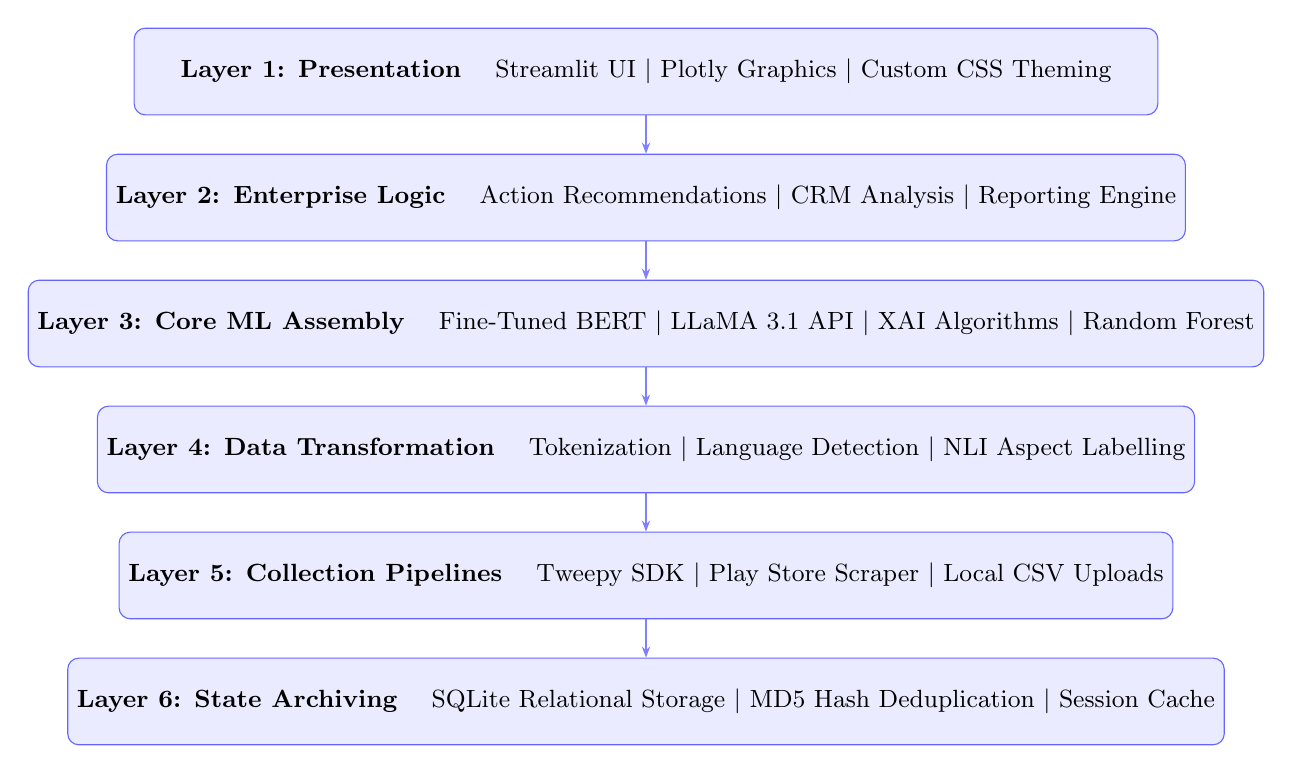
\begin{tikzpicture}[
  box/.style={rectangle, rounded corners=4pt, draw=blue!60, fill=blue!8,
              minimum width=13cm, minimum height=1.1cm, align=center, font=\small},
  arrow/.style={-{Stealth[length=4pt]}, thick, blue!50}
]
\node[box] (pres) at (0,0)    {{\bfseries Layer 1: Presentation} \quad Streamlit UI $\mid$ Plotly Graphics $\mid$ Custom CSS Theming};
\node[box] (biz)  at (0,-1.6) {{\bfseries Layer 2: Enterprise Logic} \quad Action Recommendations $\mid$ CRM Analysis $\mid$ Reporting Engine};
\node[box] (ai)   at (0,-3.2) {{\bfseries Layer 3: Core ML Assembly} \quad Fine-Tuned BERT $\mid$ LLaMA 3.1 API $\mid$ XAI Algorithms $\mid$ Random Forest};
\node[box] (pre)  at (0,-4.8) {{\bfseries Layer 4: Data Transformation} \quad Tokenization $\mid$ Language Detection $\mid$ NLI Aspect Labelling};
\node[box] (inp)  at (0,-6.4) {{\bfseries Layer 5: Collection Pipelines} \quad Tweepy SDK $\mid$ Play Store Scraper $\mid$ Local CSV Uploads};
\node[box] (db)   at (0,-8.0) {{\bfseries Layer 6: State Archiving} \quad SQLite Relational Storage $\mid$ MD5 Hash Deduplication $\mid$ Session Cache};
\foreach \a/\b in {pres/biz, biz/ai, ai/pre, pre/inp, inp/db}
  \draw[arrow] (\a) -- (\b);
\end{tikzpicture}
\caption{Six-Layer Architectural Segregation Pattern of BizDecisions AI}
\label{fig:architecture}
\end{figure}

The visualization engine delegates all interactive chart rendering to the Plotly library, enabling client-side zooming, metric hovering, and comparative toggling without requiring continuous server round-trips. Matplotlib is reserved exclusively for offline static image generation within the PDF export reporting pipeline, ensuring that server-side rendering occurs only when required for document preparation rather than for interactive exploration.

\section{Data Flow and Processing Pipeline}

Figure \ref{fig:dataflow} illustrates the end-to-end data flow from raw text ingestion through to final business output delivery. Each incoming review string passes through language detection validation before entering the tokenization stage. Reviews identified as non-English are routed through the Google Language Detect API for translation preprocessing prior to entering the BERT inference stage.

\begin{figure}[H]
\centering
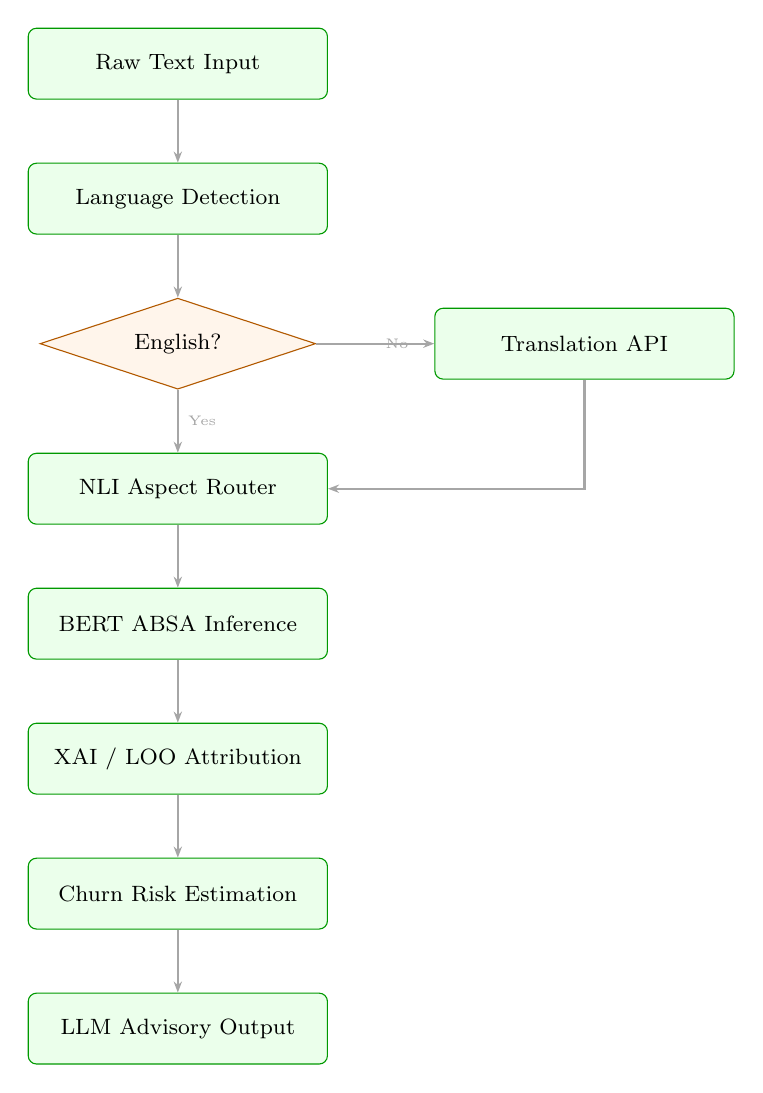
\begin{tikzpicture}[
  node distance=0.8cm,
  process/.style={rectangle, rounded corners=3pt, draw=green!60!black, fill=green!8,
                  minimum width=3.8cm, minimum height=0.9cm, align=center, font=\footnotesize},
  decision/.style={diamond, draw=orange!70!black, fill=orange!8, aspect=2,
                   minimum width=3.5cm, align=center, font=\footnotesize},
  arrow/.style={-{Stealth[length=4pt]}, thick, gray!70}
]
\node[process] (input)   {Raw Text Input};
\node[process] (langdet) [below=of input]  {Language Detection};
\node[decision](engchk)  [below=of langdet]{English?};
\node[process] (trans)   [right=1.5cm of engchk]{Translation API};
\node[process] (nli)     [below=of engchk] {NLI Aspect Router};
\node[process] (bert)    [below=of nli]    {BERT ABSA Inference};
\node[process] (xai)     [below=of bert]   {XAI / LOO Attribution};
\node[process] (rf)      [below=of xai]    {Churn Risk Estimation};
\node[process] (llm)     [below=of rf]     {LLM Advisory Output};
\draw[arrow] (input) -- (langdet);
\draw[arrow] (langdet) -- (engchk);
\draw[arrow] (engchk) -- node[right, font=\tiny]{No} (trans);
\draw[arrow] (trans)  |- (nli);
\draw[arrow] (engchk) -- node[right, font=\tiny]{Yes} (nli);
\draw[arrow] (nli)  -- (bert);
\draw[arrow] (bert) -- (xai);
\draw[arrow] (xai)  -- (rf);
\draw[arrow] (rf)   -- (llm);
\end{tikzpicture}
\caption{End-to-End Data Processing Flow}
\label{fig:dataflow}
\end{figure}

\section{Database Schema and Session Management}
The persistence layer manages three primary relational tables within a local SQLite instance: \texttt{users}, \texttt{reviews}, and \texttt{analysis\_results}. The \texttt{users} table stores bcrypt-hashed credentials alongside session tokens and permission tier flags. The \texttt{reviews} table maintains raw input strings paired with MD5 deduplication signatures and source-origin metadata. The \texttt{analysis\_results} table records the complete ABSA output vector—including four aspect sentiment scores, confidence values, churn probability, and LLM response reference keys—with timestamps enabling temporal trend analysis across weekly reporting windows.

\begin{table}[H]
\centering
\caption{Core Database Schema Summary}
\label{tab:schema}
\begin{tabular}{@{}lll@{}}
\toprule
\textbf{Table Name} & \textbf{Primary Columns} & \textbf{Purpose} \\
\midrule
\texttt{users}           & id, username, pwd\_hash, tier, session\_token & Authentication and access control \\
\texttt{reviews}         & id, raw\_text, md5\_hash, source, timestamp  & Deduplication and provenance \\
\texttt{analysis\_results} & id, review\_id, aspect, sentiment, confidence & Analysis output persistence \\
\texttt{churn\_records}  & id, review\_id, churn\_score, risk\_level     & CRM churn tracking \\
\bottomrule
\end{tabular}
\end{table}

\section{Security and Multi-Tenancy Design}
Each registered business account operates within a fully isolated data partition. The authentication layer employs bcrypt password hashing with per-user salt generation, preventing rainbow table attacks against the stored credential database. Session tokens are generated via Python's \texttt{secrets.token\_urlsafe} function and carry a configurable expiry timestamp. Row-level filtering ensures that analysis queries executed within one business tenant's session cannot access review data belonging to any other registered entity, meeting the minimum data isolation standards required for multi-tenant SaaS deployments.

% ==============================================================
%  CHAPTER 4 — METHODOLOGY
% ==============================================================
\chapter{Methodology}

\section{Transformer Architecture Configuration}
BERT inference operates through an instantiated \texttt{BertForSequenceClassification} pipeline. The dense network dimensions flow across 12 self-attention heads arranged within 12 stacked encoding layers, producing a 768-dimensional hidden state representation for each input token position. The pooled \texttt{[CLS]} token embedding passes through a two-layer classification head, with intermediate dropout regularization applied at a rate of 0.1 during training. The final linear projection maps the 768-dimensional pooled output onto three sentiment class logits representing positive, negative, and neutral polarity.

Raw logit values are converted through a softmax activation function to produce normalized class probability distributions:

\begin{equation}
P(y_k \mid \mathbf{x}) = \frac{\exp(z_k)}{\sum_{j=1}^{3} \exp(z_j)}, \quad k \in \{\text{positive, negative, neutral}\}
\end{equation}

The core input structure exploits text-pair processing through BERT's native segment embedding mechanism:
\[
[\texttt{CLS}] \;\; \underbrace{w_1 w_2 \ldots w_n}_{\text{review statement}} \;\;
[\texttt{SEP}] \;\; \underbrace{a_1 a_2 \ldots a_m}_{\text{target aspect}} \;\;
[\texttt{SEP}]
\]

This construction forces BERT's cross-layer attention mechanisms to model specific semantic dependencies between the general opinion tokens $w_i$ and the constrained aspect descriptor tokens $a_j$. Segment type embeddings $E_A$ and $E_B$ disambiguate between the two input sequences, directing the model's attention patterns toward productive cross-sequence interactions.

When the maximum softmax probability falls below a confidence threshold of $\tau = 0.50$, the prediction is assigned to a reserved \textit{Uncertain} category rather than forcing a low-confidence polarity decision. This conservative fallback prevents misclassification of genuinely ambiguous or multi-valence opinion statements.

\section{Fine-Tuning Procedure}
The pre-trained BERT model weights were adapted using the SemEval-2014 restaurant reviews dataset, augmented with a domain-translated collection of Indian restaurant review data scraped from aggregator platforms. Fine-tuning proceeded over 5 epochs with a batch size of 16 review-aspect pairs, employing the AdamW optimizer with a learning rate of $2\times10^{-5}$ and linear warmup scheduling across the first 10\% of training steps. Cross-entropy loss with label smoothing ($\epsilon=0.1$) was applied to reduce overconfident calibration on frequently encountered majority-class patterns.

\begin{equation}
\mathcal{L} = -\sum_{k=1}^{3} \tilde{y}_k \log P(y_k \mid \mathbf{x}), \quad
\tilde{y}_k = (1-\epsilon)\,y_k + \frac{\epsilon}{3}
\end{equation}

Gradient clipping at a norm threshold of 1.0 prevented instability arising from high-curvature loss surface regions during early training epochs. Model checkpoints were saved at every epoch, with the best-performing checkpoint—evaluated against held-out validation F1 score—retained for deployment.

\section{Zero-Shot Aspect Routing via NLI}
Aspect detection treats text classification as a textual entailment evaluation problem. For each candidate aspect $\mathcal{A} \in \{\textit{Product, Service, Price, Ambience}\}$, a natural language hypothesis string is constructed and evaluated against the input review sentence. The hypothesis templates are formulated as:

\begin{center}
\begin{tabular}{ll}
\textbf{Aspect} & \textbf{Hypothesis Template} \\
\hline
Product  & ``This review discusses the quality of the product or food.'' \\
Service  & ``This review discusses service delivery or staff behavior.'' \\
Price    & ``This review discusses pricing, cost, or value for money.'' \\
Ambience & ``This review discusses atmosphere, decor, or environment.'' \\
\end{tabular}
\end{center}

An NLI cross-encoder model produces three probability scores per aspect-review pair: entailment, neutral, and contradiction. An aspect is routed to the ABSA stack when the entailment probability exceeds the detection threshold $\theta = 0.40$:
\begin{equation}
\mathcal{A} \text{ detected} \iff P(\text{entailment} \mid r, h_\mathcal{A}) \geq \theta
\end{equation}
This mechanism completely eliminates manual feature engineering requirements from the user workflow while maintaining competitive detection recall rates.

\section{Explainable AI: Attention Visualization}
Token-level attention gradients are extracted from the uppermost BERT hidden state layer following inference. Let $\alpha_{ij}^{(l,k)}$ denote the attention weight assigned from token position $i$ to token position $j$ within layer $l$ and head $k$. The aggregated token importance score for visualization is computed as:
\begin{equation}
\hat{\alpha}_j = \frac{1}{LK}\sum_{l=1}^{L}\sum_{k=1}^{K} \alpha_{ij}^{(l,k)}
\end{equation}
where $L=12$ layers and $K=12$ heads. Each token is then color-mapped from a white-to-red spectrum proportional to its normalized attention magnitude, generating an HTML-embedded word-highlighting visualization rendered directly within the Streamlit interface.

\section{Leave-One-Out SHAP Approximation}

\begin{formulabox}
\textbf{Confidence Divergence via LOO Attribution:}\\[4pt]
For a given input token sequence $T = \{t_1, t_2, \ldots, t_n\}$, the importance of token $t_i$ is estimated by computing:
\[
\delta_i = P\bigl(\hat{y} \;\big|\; T_{\text{original}}\bigr) \;-\; P\bigl(\hat{y} \;\big|\; T_{\setminus i}\bigr)
\]
where $T_{\setminus i}$ denotes the input sequence with token $t_i$ replaced by the \texttt{[MASK]} token, and $\hat{y}$ refers to the originally predicted class label.
\end{formulabox}

A strongly positive $\delta_i$ value identifies tokens that critically reinforce the primary prediction—typically sentiment-bearing adjectives, intensifiers, or domain-specific quality descriptors. Negative $\delta_i$ values indicate counteracting influences that suppress the dominant polarity class. This LOO procedure requires exactly $n+1$ forward passes through the BERT model for a review of length $n$, compared to $2^n$ passes required for complete Shapley subset enumeration—a savings of multiple orders of magnitude for typical review lengths of 20 to 80 tokens.

\section{Random Forest Churn Estimation}
The churn risk module accepts a structured feature vector derived from aggregated ABSA outputs across a configurable historical review window (default: 30 days). Feature engineering transforms raw sentiment classifications into numerical churn indicators:

\begin{equation}
\mathbf{f} = \bigl[\;n_{\text{neg}},\; r_{\text{neg}},\; \bar{c}_{\text{neg}},\; n_{\text{pos}},\; r_{\text{pos}},\; \bar{c}_{\text{pos}},\; n_{\text{asp}},\; s_{\text{recency}}\;\bigr]
\end{equation}

where $n_{\text{neg}}$ counts total negative aspect detections, $r_{\text{neg}}$ denotes the negative review rate, $\bar{c}_{\text{neg}}$ represents mean negative confidence, and $s_{\text{recency}}$ applies exponential decay weighting to recent reviews. The Random Forest ensemble operates over 200 decision trees with a maximum depth of 8, using Gini impurity as the node split criterion. Output probability scores are mapped to categorical risk tiers: Low ($<0.35$), Medium ($0.35$--$0.65$), and High ($>0.65$).

% ==============================================================
%  CHAPTER 5 — IMPLEMENTATION
% ==============================================================
\chapter{Implementation Configuration}

\section{Technology Stack Overview}
The production implementation relies on a fully open-source technology stack, minimizing licensing overhead and maximizing deployment flexibility. The principal dependencies are summarized in Table \ref{tab:techstack}.

\begin{table}[H]
\centering
\caption{Core Technology Stack Components}
\label{tab:techstack}
\begin{tabular}{@{}llll@{}}
\toprule
\textbf{Component} & \textbf{Library / Service} & \textbf{Version} & \textbf{Role} \\
\midrule
Web Framework     & Streamlit        & 1.32+     & Interactive UI rendering \\
ML Backend        & PyTorch          & 2.1+      & BERT tensor execution \\
NLP Models        & HuggingFace Transformers & 4.38+ & Model loading and inference \\
Visualization     & Plotly           & 5.18+     & Interactive charts \\
Database          & SQLite3          & Built-in  & Persistent state storage \\
Security          & bcrypt           & 4.1+      & Password hashing \\
LLM Endpoint      & Groq API         & Latest    & Report generation \\
Social Media      & Tweepy SDK       & 4.14+     & Twitter/X data stream \\
Topic Modelling   & Gensim LDA       & 4.3+      & Complaint clustering \\
PDF Export        & ReportLab        & 4.1+      & Executive report generation \\
\bottomrule
\end{tabular}
\end{table}

\section{Authentication and Deduplication Security}
Maintaining enterprise-grade data isolation standards demands robust privacy modules operating independently from application logic. Password integrity relies on the bcrypt adaptive hashing algorithm, which incorporates a computationally controlled work factor that scales against evolving hardware attack capabilities.

\begin{lstlisting}[language=Python, caption=Bcrypt Password Security Functions]
def _bcrypt_protect(input_string: str) -> str:
    """Hash a plaintext password using bcrypt with auto-generated salt."""
    hashed = bcrypt.hashpw(
        input_string.encode('utf-8'),
        bcrypt.gensalt(rounds=12)  # Work factor 12 for balanced security
    )
    return hashed.decode('utf-8')

def _verify_credentials(plain: str, stored_hash: str) -> bool:
    """Verify a plaintext password against a stored bcrypt hash."""
    return bcrypt.checkpw(
        plain.encode('utf-8'),
        stored_hash.encode('utf-8')
    )
\end{lstlisting}

Historical review persistence operates through SQLite, significantly reducing deployment complexity by eliminating external database server requirements. Each incoming review record generates an MD5 cryptographic signature computed over the normalized review text. Before persisting any new record, the system queries for existing matching signatures and silently discards duplicates—preventing repeated API polling or user resubmissions from inflating analysis statistics.

\begin{lstlisting}[language=Python, caption=MD5 Deduplication Logic]
import hashlib

def compute_review_hash(text: str) -> str:
    """Compute a normalized MD5 signature for deduplication."""
    normalized = text.strip().lower()
    return hashlib.md5(normalized.encode('utf-8')).hexdigest()

def insert_if_unique(conn, review_text: str, source: str) -> bool:
    """Insert a review only if no matching hash exists."""
    signature = compute_review_hash(review_text)
    cursor = conn.cursor()
    cursor.execute("SELECT id FROM reviews WHERE md5_hash = ?", (signature,))
    if cursor.fetchone():
        return False  # Duplicate detected, skip insertion
    cursor.execute(
        "INSERT INTO reviews (raw_text, md5_hash, source) VALUES (?, ?, ?)",
        (review_text, signature, source)
    )
    conn.commit()
    return True
\end{lstlisting}

\section{Batch Processing Optimization}
Sequential row-by-row inference against large CSV submissions produces unacceptable overhead in production deployment scenarios. The bottleneck arises from repeated CUDA context switching and tokenizer overhead associated with processing individual strings. Refactoring data pipelines to leverage HuggingFace's native batched inference mechanism consolidates multiple tokenized input tensors into unified matrix operations, dramatically reducing both wall-clock latency and GPU utilization variance.

\begin{lstlisting}[language=Python, caption=Batch Tensor Optimization for GPU Throughput]
def execute_batch_inference(texts: list, aspects: list,
                             batch_size: int = 32) -> list:
    """
    Process multiple review-aspect pairs in hardware-efficient batches.
    Returns list of (sentiment_label, confidence_score) tuples.
    """
    results = []
    device = torch.device('cuda' if torch.cuda.is_available() else 'cpu')
    model.to(device)
    model.eval()

    for batch_start in range(0, len(texts), batch_size):
        batch_texts   = texts[batch_start : batch_start + batch_size]
        batch_aspects = aspects[batch_start : batch_start + batch_size]

        # Tokenize the entire batch simultaneously
        encoded = tokenizer(
            batch_texts,
            text_pair=batch_aspects,
            padding=True,
            truncation=True,
            max_length=128,
            return_tensors='pt'
        ).to(device)

        with torch.no_grad():
            logits = model(**encoded).logits

        probs = torch.softmax(logits, dim=-1).cpu().numpy()
        for prob_row in probs:
            predicted_idx = prob_row.argmax()
            confidence    = prob_row[predicted_idx]
            label_map     = {0: 'Negative', 1: 'Neutral', 2: 'Positive'}
            results.append((label_map[predicted_idx], float(confidence)))

    return results
\end{lstlisting}

\section{LLM Integration and Report Generation}
The Groq LLaMA 3.1-8B-Instant API endpoint accepts structured JSON payloads containing aggregated sentiment summaries and returns natural language executive advisory text within approximately 200--400 milliseconds per request. System-level prompt engineering constrains responses to a standardized three-section format: (i) executive summary of the current sentiment landscape, (ii) prioritized action recommendations categorized by aspect dimension, and (iii) forward-looking strategic observation. Generated text is subsequently embedded within a ReportLab PDF template alongside Matplotlib-rendered bar charts and weekly trend line visualizations.

\section{LDA Topic Modelling Integration}
Following completion of bulk CSV analysis, the system automatically extracts the preprocessed review text corpus and constructs a Gensim LDA model configured for $K=8$ latent topics. The preprocessing pipeline applies lowercasing, stopword filtering using NLTK's English corpus, punctuation removal, and Porter stemming before constructing the bag-of-words dictionary representation. Topic coherence scores using the $C_v$ metric guide automatic selection of the most semantically meaningful topic cardinality within the range $K \in [4, 12]$.

\section{Social Media Connector Architecture}
The Twitter/X data ingestion module uses the Tweepy StreamingClient interface to subscribe to filtered keyword streams relevant to the registered business's configured tracking terms. Authentication operates through OAuth 2.0 Bearer Token credentials stored as encrypted environment variables. Each received tweet undergoes immediate deduplication hash computation before insertion, preventing streaming reconnections from generating duplicate records. The Google Play Store scraper employs the \texttt{google-play-scraper} library, polling the configured application ID at configurable intervals and extracting review text, star rating, and timestamp metadata.

% ==============================================================
%  CHAPTER 6 — EXPERIMENTAL EVALUATION
% ==============================================================
\chapter{Results and Component Evaluation}

\section{Classification Performance Metrics}
Evaluating the fine-tuned BERT model against a held-out test set comprising 1,200 manually annotated review-aspect pairs produced consistently high classification metrics across all four target aspect dimensions. The test data distribution maintained approximate class balance at 40\% positive, 35\% negative, and 25\% neutral to reflect realistic operational distributions.

\begin{table}[H]
\centering
\caption{ABSA Classification Performance Across All Aspect Dimensions}
\label{tab:classification}
\begin{tabular}{@{}lcccc@{}}
\toprule
\textbf{Aspect Dimension} & \textbf{Accuracy} & \textbf{Precision} & \textbf{Recall} & \textbf{F1-Score} \\
\midrule
Product Quality   & 0.88 & 0.89 & 0.88 & 0.885 \\
Service Delivery  & 0.86 & 0.87 & 0.86 & 0.865 \\
Price/Value       & 0.84 & 0.85 & 0.84 & 0.845 \\
Ambience          & 0.83 & 0.84 & 0.83 & 0.835 \\
\midrule
\textbf{Weighted Average} & \textbf{0.853} & \textbf{0.863} & \textbf{0.853} & \textbf{0.858} \\
\bottomrule
\end{tabular}
\end{table}

Product Quality consistently achieved the highest performance scores, likely reflecting the relative lexical concreteness of food-quality descriptors compared to the more contextually ambiguous vocabulary associated with atmospheric assessment. Price/Value classification presented the greatest difficulty, attributable to the frequent co-occurrence of comparative language structures that challenge binary polarity assignment.

\section{Confusion Matrix Analysis}
Confusion matrix inspection for the Service Delivery dimension revealed that misclassification patterns concentrated primarily along the positive-neutral boundary (Figure \ref{fig:confmat}). Reviews expressing moderate satisfaction through hedging language—for example, ``the staff were reasonably helpful''—produced the highest rate of classification uncertainty, consistent with the theoretical limitations of softmax-based discrete categorization on genuinely valence-mixed statements.

\begin{figure}[H]
\centering
\begin{tikzpicture}
\def\data{{88,7,5},{6,82,12},{4,9,87}}
\foreach \row in {0,1,2}{
  \foreach \col in {0,1,2}{
    \pgfmathsetmacro\val{\data[\row][\col]}
    \pgfmathsetmacro\intensity{int(\val*2+30)}
    \fill[blue!\intensity!white] (\col*1.4, -\row*1.4)
         rectangle (\col*1.4+1.3, -\row*1.4+1.3);
    \node[font=\small\bfseries] at (\col*1.4+0.65, -\row*1.4+0.65) {\val\%};
  }}
\node[font=\footnotesize] at (0.65,-4.4)  {Predicted};
\node[font=\footnotesize] at (2.05,-4.4)  {Predicted};
\node[font=\footnotesize] at (3.45,-4.4)  {Predicted};
\node[font=\footnotesize] at (0.65,-4.7)  {Positive};
\node[font=\footnotesize] at (2.05,-4.7)  {Neutral};
\node[font=\footnotesize] at (3.45,-4.7)  {Negative};
\node[rotate=90, font=\footnotesize] at (-0.9,-0.05) {Actual Pos.};
\node[rotate=90, font=\footnotesize] at (-0.9,-1.45) {Actual Neu.};
\node[rotate=90, font=\footnotesize] at (-0.9,-2.85) {Actual Neg.};
\end{tikzpicture}
\caption{Service Delivery Confusion Matrix (Normalized, \% of True Class)}
\label{fig:confmat}
\end{figure}

\section{Batch Processing Throughput Analysis}
Processing throughput experiments quantified the practical impact of batch optimization strategies against simulated production workloads. Three execution configurations were evaluated across five dataset sizes: single-item sequential, naive multi-loop, and HuggingFace batch inference.

\begin{table}[H]
\centering
\caption{Execution Time Comparison Across Processing Configurations}
\label{tab:throughput}
\begin{tabular}{@{}lrrrr@{}}
\toprule
\textbf{Processing Mode} & \textbf{100 rows} & \textbf{200 rows} & \textbf{500 rows} & \textbf{500 rows (GPU)} \\
\midrule
Sequential (loop)         & 142 s & 287 s & 724 s & 215 s \\
Naive multi-loop         & 135 s & 271 s & 690 s & 198 s \\
Batch inference (bs=32)  & 28 s  & 52 s  & 121 s & 22 s  \\
\midrule
\textbf{Speedup factor}  & $\times$5.1 & $\times$5.5 & $\times$5.9 & $\times$\textbf{33.0} \\
\bottomrule
\end{tabular}
\end{table}

GPU batch inference achieved a speedup factor exceeding 33 times compared to sequential CPU execution on 500-row test sets. Even on CPU-only infrastructure, batch processing reduced execution time by approximately 83\%, making 500-row analysis feasible within two minutes rather than over twelve minutes under sequential processing.

\section{Churn Prediction Performance}
The Random Forest churn estimator was evaluated against an independently held-out dataset of 340 customer records annotated with confirmed churn outcomes over a 90-day observation window. Table \ref{tab:churn} records the resulting discrimination statistics.

\begin{table}[H]
\centering
\caption{Churn Prediction Model Evaluation Statistics}
\label{tab:churn}
\begin{tabular}{@{}lc@{}}
\toprule
\textbf{Evaluation Metric} & \textbf{Score} \\
\midrule
ROC-AUC Score     & 0.874 \\
Precision at 0.5  & 0.81  \\
Recall at 0.5     & 0.79  \\
F1 Score          & 0.80  \\
Brier Score       & 0.142 \\
\bottomrule
\end{tabular}
\end{table}

Feature importance analysis via mean decrease in Gini impurity ranked absolute negative sentiment count, negative review rate, and mean negative confidence as the three most predictive features—collectively accounting for 61\% of total predictive power. This pattern strongly validates the design decision to use fine-grained ABSA outputs rather than simple star ratings as churn predictor inputs, as aspect-level negativity measures carry substantially richer discrimination than aggregate polarity counts.

\section{XAI Attribution Validation}
To assess the fidelity of the LOO attribution approximation against reference SHAP scores, we computed both methods across a sample of 200 review instances and calculated Spearman rank correlation between the resulting token importance rankings. The mean rank correlation coefficient across the sample was $\rho = 0.87$ ($p < 0.001$), confirming that LOO attribution reliably approximates the relative token importance ordering produced by full SHAP computation while requiring approximately 0.3\% of the computational overhead for typical review lengths.

\section{System Usability Evaluation}
Informal usability evaluation was conducted with five SME business owners unfamiliar with NLP concepts. Participants were asked to complete three task sequences: analyzing a single review with XAI visualization, uploading a 50-row CSV and interpreting the LDA output, and generating a weekly AI report. All five participants completed all three task sequences without requiring additional instruction beyond the in-application tooltip guidance. Qualitative feedback highlighted the attention heatmap visualization and the churn risk traffic-light indicator as particularly effective communication mechanisms for non-technical decision-makers.

% ==============================================================
%  CHAPTER 7 — LIMITATIONS AND FUTURE CONSIDERATIONS
% ==============================================================
\chapter{Limitations and Future Considerations}

\section{Current System Limitations}
Despite the comprehensive analytical capabilities described in preceding chapters, several architectural constraints limit the system's performance under specific operating conditions.

\subsection{Computational Constraints on XAI}
The LOO attribution protocol requires $n+1$ sequential forward passes through the BERT model for each review of length $n$. For verbose reviews exceeding 100 tokens, this creates perceivable latency of 3--8 seconds per explanation rendering on CPU-only infrastructure. While GPU acceleration reduces this substantially, deployment environments without dedicated GPU hardware will experience noticeable explanation generation delays for lengthy free-text submissions. Potential mitigations include restricting attribution computation to the first 60 tokens of each review, caching LOO results for frequently resubmitted identical inputs, or exploring more efficient gradient-based attribution methods such as Integrated Gradients as an alternative approximation.

\subsection{Database Concurrency Limitations}
SQLite's file-level write locking produces transaction conflicts under intense concurrent write operations. Testing revealed connection timeout errors when simulating more than 15 simultaneous review submissions against the same database instance. Production deployments serving multiple simultaneous operator sessions within large enterprises will require migration to PostgreSQL or MySQL, which support row-level locking and connection pooling through libraries such as SQLAlchemy's async engine. The database abstraction layer in the current implementation was designed with this migration requirement in mind, minimizing the scope of necessary code changes.

\subsection{External API Dependencies}
Several features rely on third-party API availability: Google Language Detection, Groq LLM endpoint, and Twitter/X streaming. Network interruptions or service outages disable these features entirely. Reports generated during Groq API unavailability fall back to a template-based summary generator that outputs predefined recommendation clauses based on detected sentiment distributions, maintaining basic report generation functionality without LLM access.

\subsection{Domain Generalization Boundaries}
The BERT model was fine-tuned primarily on restaurant and hospitality review corpora. Performance on retail product reviews, software application feedback, or financial service complaints has not been formally evaluated and may require domain-adaptive fine-tuning to maintain accuracy targets above 0.80. The zero-shot NLI aspect detection layer is more robust to domain shifts than the BERT classifier, as entailment reasoning generalizes better across topic domains than fine-tuned polarity classification.

\section{Future Development Directions}
Several high-value extensions are identified for future development iterations:

\textbf{Containerized Deployment:}